% =====================================================================
%  Figure panels for: A Residual Algebra for Catalytic Composition
%  Captions quote measured values; see validation/results/panel_stats.json
% =====================================================================

\begin{figure*}[!htbp]
    \centering
    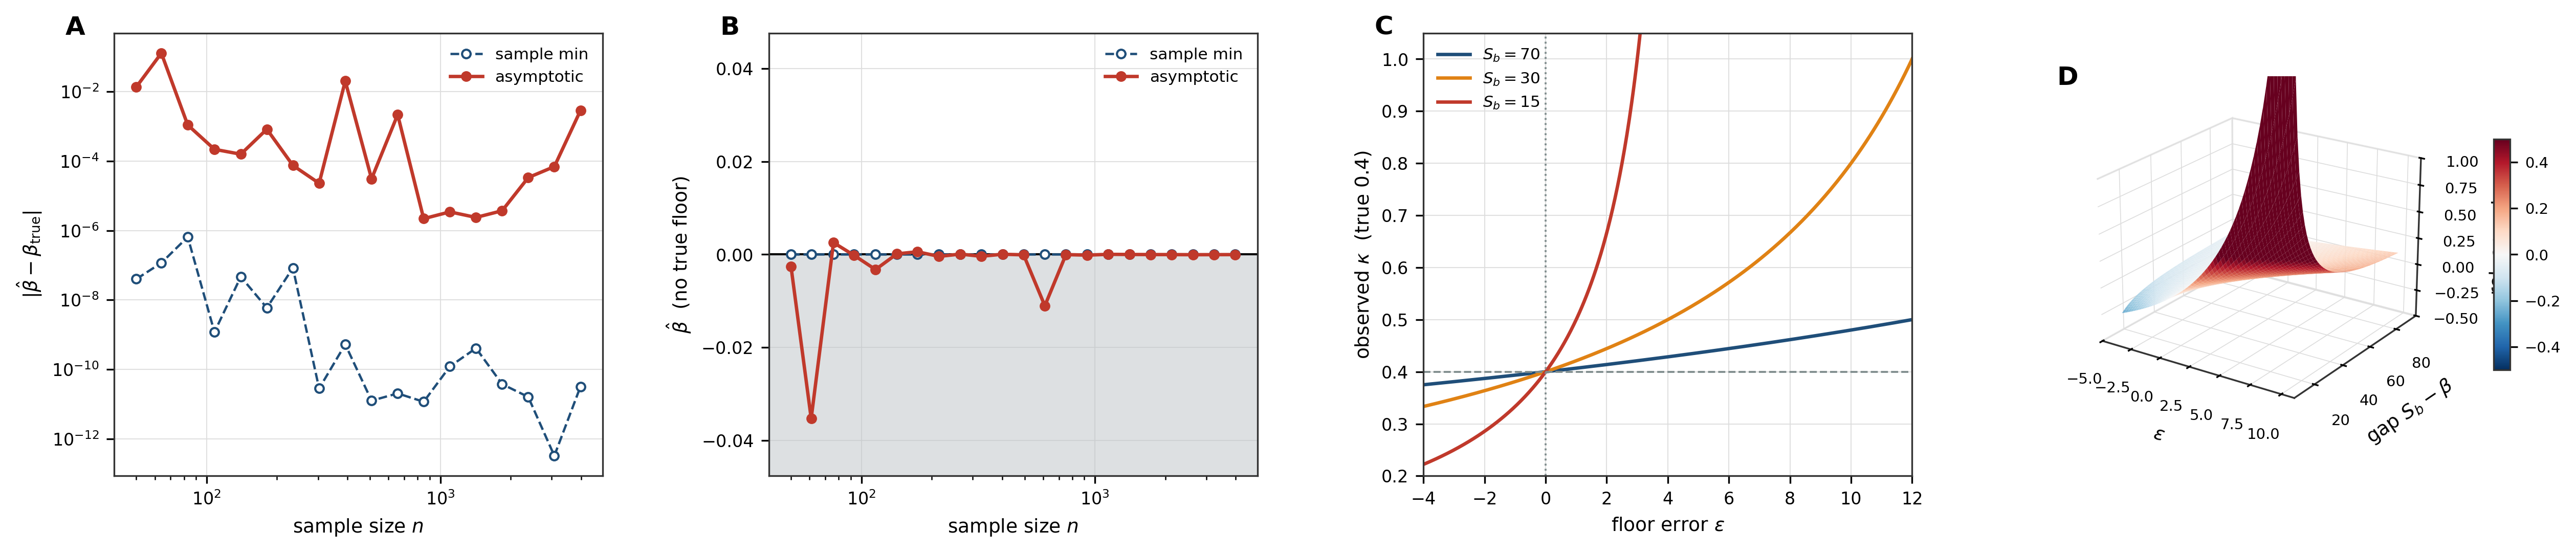
\includegraphics[width=\textwidth]{figures/panel_1_floor.png}
    \caption{\textbf{The floor: only one of the two estimators is capable of contradicting a positivity claim.}
    All quantities are computed on synthetic processes whose true floor is known by construction, so estimator error is measured against a fact rather than inferred. The generating density places most of its mass near the floor (cubic in a uniform draw), which is the regime in which the two estimators are hardest to tell apart, and is therefore the conservative choice.
    (\textbf{A})~Absolute error of both estimators against sample size on a process with true floor $\flo=10$, log--log axes, $18$ sample sizes spanning $n=50$ to $n=3981$. The sample minimum is the more accurate of the two throughout, with median error $2.6\times10^{-10}$ against $1.2\times10^{-4}$ for the asymptotic intercept. We record this because it runs against the paper's recommendation and is a genuine property of this generator: when the density piles up at the floor, the smallest of many draws lands very close to it. Accuracy is not the property at issue, and panel~(B) is where the two estimators separate.
    (\textbf{B})~Signed estimate on a process with \emph{no} floor, $22$ sample sizes. The sample minimum returns a strictly positive value at every one of them, ranging from $9.8\times10^{-6}$ down to $6.1\times10^{-17}$ but never reaching or crossing zero; the asymptotic intercept is negative at $16$ of the $22$ sizes, reaching $-3.5\times10^{-2}$. This is \Cref{rem:floor-empirical}: an estimator bounded below by zero cannot return evidence against $\flo>0$, however precise it is, so its positivity confirms nothing. The shaded band is the region a falsifying observation must reach, and only one estimator enters it.
    (\textbf{C})~Observed catalytic power against an error $\eps$ in the assumed floor, for events acting at three distances above it, true power $0.4$ in every case. An overestimate of $\eps=2$ inflates a near-floor event ($S_b=15$) to $0.667$ while a distant event ($S_b=70$) moves only to $0.414$. This is \Cref{prop:floor-sensitivity} and it compounds the bias of panel~(B): the sample minimum is an upper bound on the infimum, so its error has the sign that inflates, and inflates most for exactly the events an experimenter is most interested in.
    (\textbf{D})~The relative error $\eps/(S_b-\flo-\eps)$ as a surface over floor error and gap. The surface is flat and near zero across the large-gap region and turns sharply upward as the gap closes on $\eps$, reaching $5.0$ at the corner where the assumed floor sits within two units of the pre-event state. The asymmetry about $\eps=0$ is the substantive content: underestimating the floor is benign, overestimating it is not, and the sample minimum errs in the second direction by construction.}
    \label{fig:panel1}
\end{figure*}

\begin{figure*}[!htbp]
    \centering
    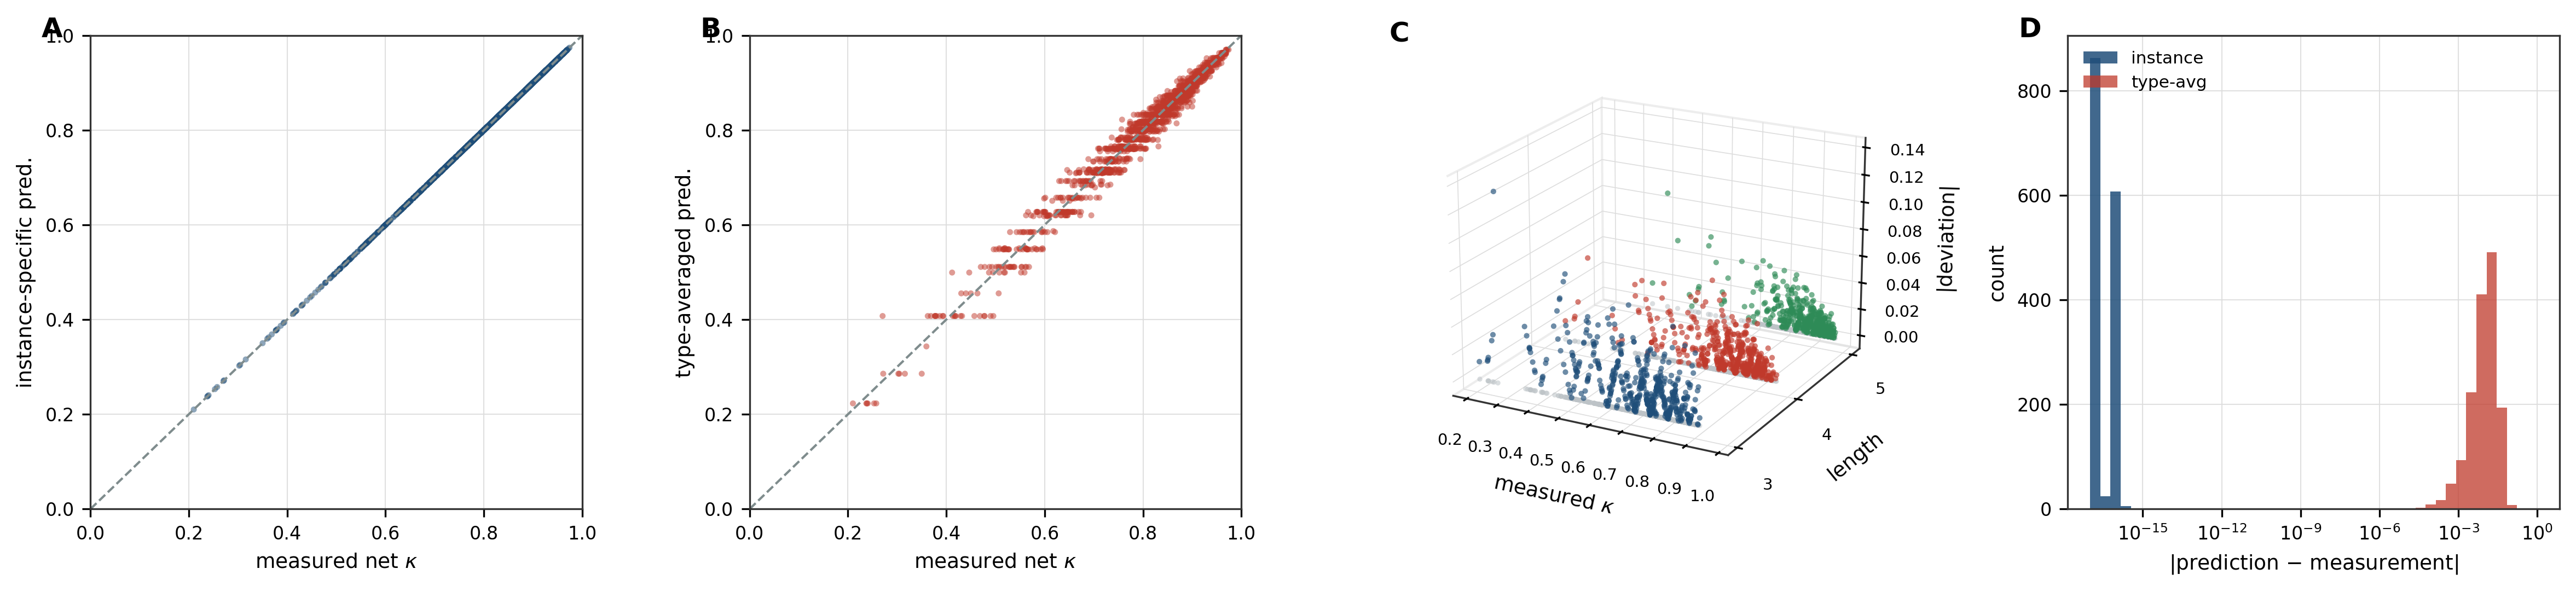
\includegraphics[width=\textwidth]{figures/panel_2_telescoping.png}
    \caption{\textbf{The natural test of the composition law is an algebraic identity, and reports perfect agreement on data generated by any process whatsoever.}
    $1500$ cascades of length $3$ to $5$, drawn from the separated regime; measured net powers span $0.210$ to $0.974$. The two predictions plotted in (A) and (B) differ only in how the constituent powers are estimated---from the same cascade, or from the population of events of that type---and in nothing else.
    (\textbf{A})~Instance-specific multiplicative prediction against measured net power. Every point lies on the diagonal: the maximum absolute deviation over all $1500$ cascades is $2.22\times10^{-16}$, one unit in the last place of double precision, and the median deviation is exactly zero. This is \Cref{thm:telescoping}. The agreement is not evidence for the multiplicative law, because the two axes are the same algebraic expression evaluated twice; by \Cref{cor:no-null} the same figure would be produced by data from a process violating every claim in the paper.
    (\textbf{B})~The identical axes under type-averaged estimation. The scatter is real: maximum deviation $0.137$, median $1.06\times10^{-2}$, $r=0.988$, $\mathrm{RMSE}=0.0199$. The test now has a null it could fail (\Cref{thm:nondegenerate}), and the fit it reports is a claim about the process rather than about the algebra. The visible upward curvature at low measured power is the first-order behaviour predicted by \Cref{prop:bias}, in which within-type deviations enter amplified by $1/(1-\bar\kap)$.
    (\textbf{C})~Absolute deviation from measurement against measured power and cascade length. The instance-specific deviations (grey) lie flat on the floor of the vertical axis at every length; the type-averaged deviations (coloured by length) rise away from it and spread further at length $5$ than at length $3$, since the deviations of \Cref{prop:bias} accumulate additively over the events composed.
    (\textbf{D})~Distribution of the same two deviation sets on a logarithmic axis. They are separated by roughly sixteen orders of magnitude: the instance-specific mass sits against the machine-epsilon bound, the type-averaged mass occupies $10^{-3}$ to $10^{-1}$. The gap is the whole methodological content of \Cref{sec:telescoping}, and its size is the reason the degenerate test is easy to run without noticing: an $r$ of exactly $1.000$ looks like an unusually strong result rather than an arithmetic tautology.}
    \label{fig:panel2}
\end{figure*}

\begin{figure*}[!htbp]
    \centering
    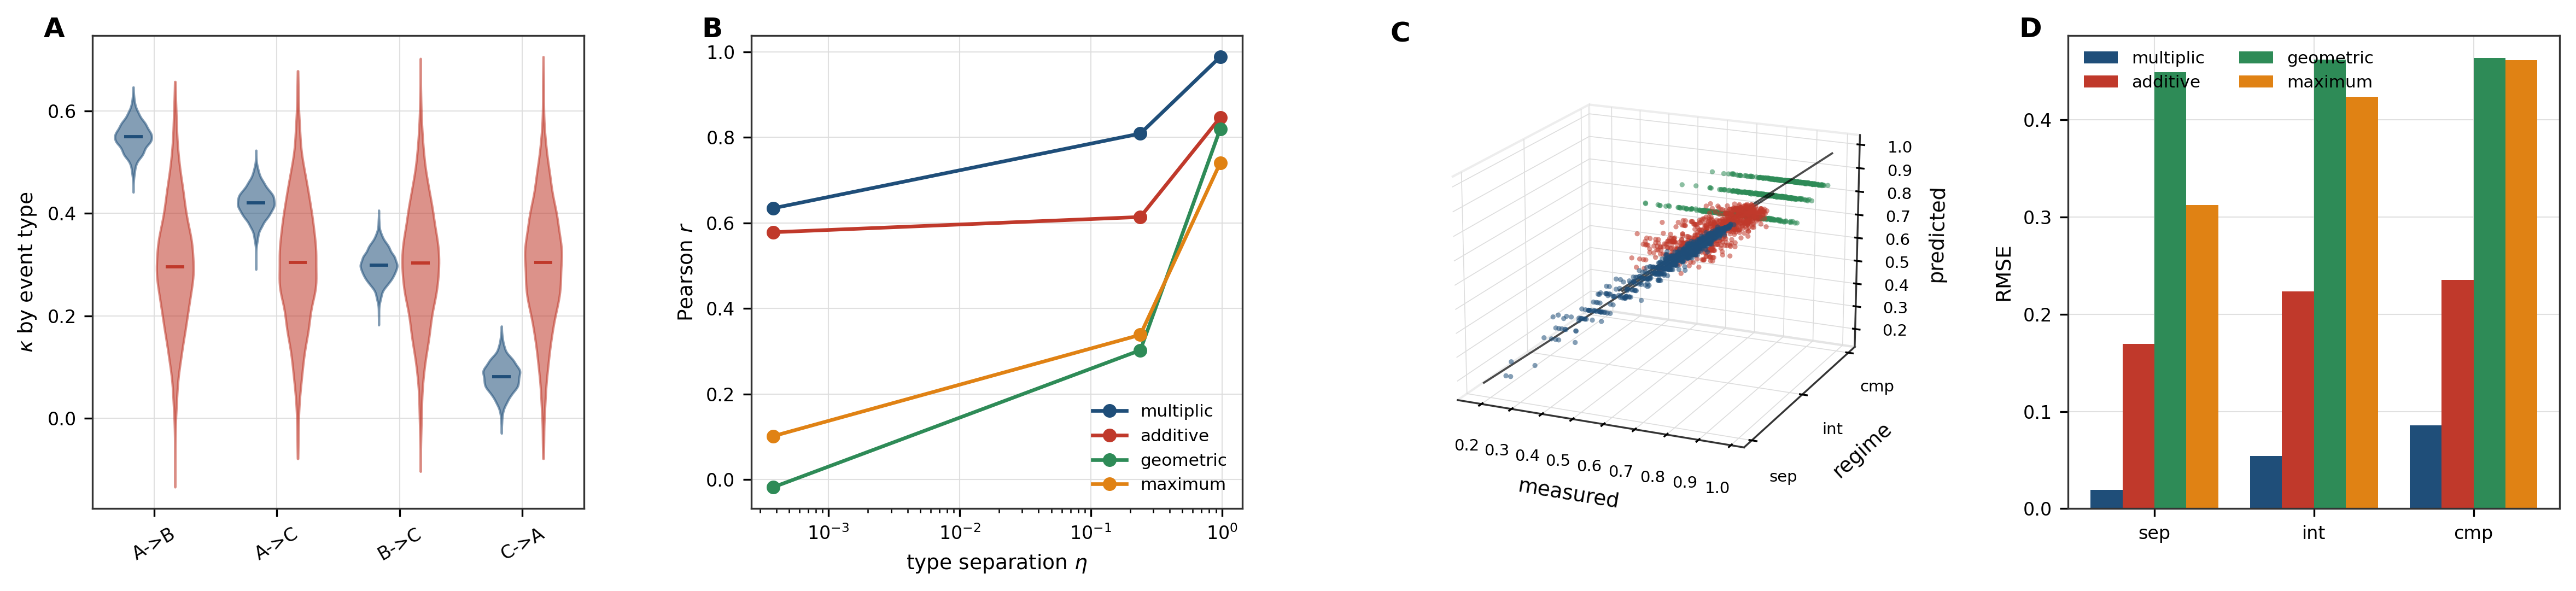
\includegraphics[width=\textwidth]{figures/panel_3_separation.png}
    \caption{\textbf{Type separation governs whether the corrected test can adjudicate, and the laws degrade at different rates rather than together.}
    Three regimes of $3000$ cascades each, differing only in how far apart the four event types' mean powers are placed and how widely instances of a type disperse around them. Separation is reported as $\eta$ (\Cref{def:variance}); the regimes realise $\eta=0.971$, $0.239$ and $3.8\times10^{-4}$, spanning type-mean spreads of $0.469$, $0.121$ and $0.006$ against within-type dispersions of $0.030$, $0.080$ and $0.120$.
    (\textbf{A})~Within-type distributions of $\kap$ for the separated (blue) and compressed (red) regimes. In the separated regime the four medians are visibly distinct and each distribution is narrow; in the compressed regime the medians coincide to three significant figures while the distributions widen to overlap almost completely. The compressed regime is not a noisier version of the separated one---it is one in which the typing has stopped carrying information about the power, which is the condition \Cref{prop:degeneracy} concerns.
    (\textbf{B})~Pearson $r$ between type-averaged prediction and measurement for the four laws, against $\eta$ on a logarithmic axis. The laws do not degrade together. Across the four-orders-of-magnitude fall in $\eta$ the multiplicative law declines from $0.988$ to $0.634$, while the geometric-mean law falls from $0.819$ to $-0.018$ and the maximum law from $0.740$ to $0.102$. \Cref{rem:graceful} identifies the residual correlation as an artefact of cascade-length variation: at a common type mean the multiplicative prediction $1-(1-\bar\kap)^n$ still tracks $n$, whereas the maximum law is constant in $n$. A non-trivial $r$ at low $\eta$ is therefore not evidence that the typing is correct, which is why $\eta$ must be reported alongside it.
    (\textbf{C})~Predicted against measured net power for the multiplicative law in each regime, with the identity line drawn in each plane. The scatter widens monotonically as $\eta$ falls while remaining centred on the identity, showing that compression degrades precision without introducing bias.
    (\textbf{D})~RMSE by law and regime. The multiplicative law attains the lowest error in all three ($0.020$, $0.054$, $0.086$) and the ordering of the remaining three is not stable across regimes: the additive law is second everywhere, but the geometric-mean and maximum laws exchange places between the separated and intermediate regimes. Only the first of these facts is a finding about the data; the second is a caution against reading a ranking off a single regime.}
    \label{fig:panel3}
\end{figure*}

\begin{figure*}[!htbp]
    \centering
    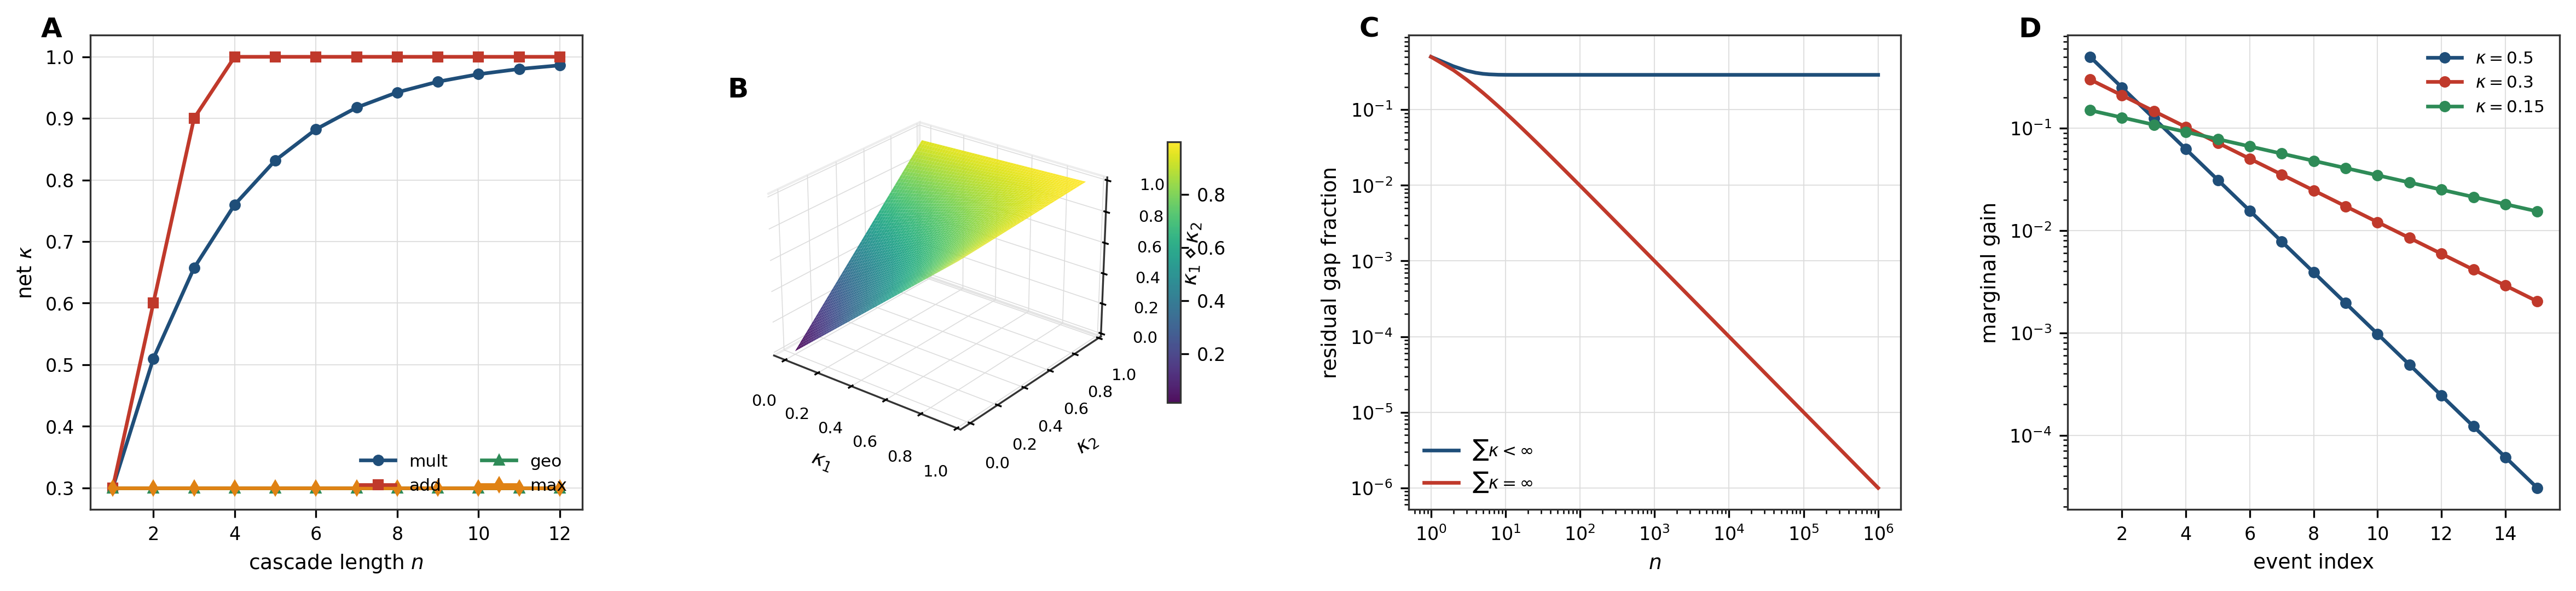
\includegraphics[width=\textwidth]{figures/panel_4_composition.png}
    \caption{\textbf{Composition geometry: the law saturates without attaining, and convergence is decided by summability rather than by magnitude.}
    All four charts evaluate the algebra directly rather than sampling it, so the curves are the theorems and not estimates of them.
    (\textbf{A})~The four composition laws as functions of cascade length at fixed per-event power $\kap=0.3$. The additive law saturates at unity by $n=4$ and is thereafter constant, asserting that four events of power $0.3$ close the gap completely; the multiplicative law reaches $0.986$ at $n=12$ and approaches unity without attaining it, which is \Cref{cor:not-attained}. The geometric-mean law reduces to $\kap$ at constant power and therefore coincides exactly with the maximum law; it is drawn dashed and heavier so that the coincidence is visible rather than one curve concealing the other.
    (\textbf{B})~The composition surface $1-(1-\kap_1)(1-\kap_2)$ over the unit square. It is symmetric about the diagonal, which is the commutativity of \Cref{cor:structure}, and rises to unity along both edges where either argument approaches $1$, which is the absorbing element. The surface is strictly below the plane $\kap_1+\kap_2$ everywhere off the axes, the strict form of the bound in \Cref{prop:competitors}.
    (\textbf{C})~Residual gap fraction against cascade length for a summable and a non-summable sequence of powers, log--log axes to $n=10^6$. With $\kap_i=2^{-(i+1)}$ the fraction stabilises at $0.2888$ and does not move thereafter: the uncertainty converges, but to a value strictly above the floor. With $\kap_i=1/(i+2)$ it follows the exact closed form $1/(n+1)$, reaching $1.0\times10^{-6}$. Both branches of \Cref{thm:convergence} are shown; note that the divergent case converges only harmonically, so a stopping criterion phrased as ``residual below a fixed tolerance at finite $n$'' would be testing the tolerance and not the theorem.
    (\textbf{D})~Marginal contribution of the $n$th event, $\kap(1-\kap)^{n-1}$, logarithmic axis. At $\kap=0.5$ the tenth event contributes $9.8\times10^{-4}$; at $\kap=0.15$ it still contributes $3.5\times10^{-2}$. The lines are straight on this axis because the decay is exactly geometric (\Cref{prop:diminishing}), and they cross: a cascade of weak events eventually contributes more per event than a cascade of strong ones, because the strong cascade has already consumed the gap it was closing.}
    \label{fig:panel4}
\end{figure*}
